% Created 2015-10-16 Fri 21:59
\documentclass[11pt]{article}
\usepackage[utf8]{inputenc}
\usepackage[T1]{fontenc}
\usepackage{fixltx2e}
\usepackage{graphicx}
\usepackage{longtable}
\usepackage{float}
\usepackage{wrapfig}
\usepackage{rotating}
\usepackage[normalem]{ulem}
\usepackage{amsmath}
\usepackage{textcomp}
\usepackage{marvosym}
\usepackage{wasysym}
\usepackage{amssymb}
\usepackage{capt-of}
\usepackage[hidelinks]{hyperref}
\tolerance=1000
\usepackage[utf8]{inputenc}
\usepackage[usenames,dvipsnames]{color}
\usepackage{commath}
\usepackage{listings}
\usepackage{color}
\usepackage{enumerate}
\usepackage{minted}
\usepackage{standalone}
\usepackage{calc}
\usepackage{./latex/doxygen}
\usemintedstyle{perldoc}
\hypersetup{urlcolor=blue}
\hypersetup{colorlinks,urlcolor=blue}
\setlength{\parskip}{16pt plus 2pt minus 2pt}
\renewcommand{\arraystretch}{1.6}
\definecolor{codebg}{rgb}{0.96,0.99,0.8}
\newcommand{\+}{\discretionary{\mbox{\scriptsize$\hookleftarrow$}}{}{}}
\author{Oleg Sivokon}
\date{\textit{<2015-10-15 Thu>}}
\title{Selected Project Euler Exercises}
\hypersetup{
 pdfauthor={Oleg Sivokon},
 pdftitle={Selected Project Euler Exercises},
 pdfkeywords={Project Euler, Assignment, Firmitas},
 pdfsubject={Selected Project Euler Exercise, Assignment for Firmitas CS},
 pdfcreator={Emacs 25.0.50.1 (Org mode 8.3beta)}, 
 pdflang={English}}
\begin{document}

\maketitle
\tableofcontents

\newpage

\section{Foreword}
\label{sec:orgheadline1}
\section{Exercises}
\label{sec:orgheadline18}
\subsection{1000-digits Fibonacci number PE-25}
\label{sec:orgheadline5}
\subsubsection{Problem Statement}
\label{sec:orgheadline2}
The Fibonacci sequence is defined by the recurrence relation:

\begin{equation*}
  F_n = F_{n-1} + F_{n-2},\; \textit{where}\; F_1 = 1\; \textit{and} \; F_2 = 1\;.
\end{equation*}


Hence the first 12 terms will be:

\begin{align*}
  F_1    &= 1   \\
  F_2    &= 1   \\
  F_3    &= 2   \\
  F_4    &= 3   \\
  F_5    &= 5   \\
  F_6    &= 8   \\
  F_7    &= 13  \\
  F_8    &= 21  \\
  F_9    &= 34  \\
  F_{10} &= 55  \\
  F_{11} &= 89  \\
  F_{12} &= 144
\end{align*}


The \(12^{th}\) term, \(F_{12}\), is the first term to contain three digits.

What is the index of the first term in the Fibonacci sequence 
to contain 1000 digits?

\subsubsection{Discussion}
\label{sec:orgheadline3}
Start with some initial guess: \(fib(1000)\) and double the size until we find
a number with more than 1000 digits once done, subtract the half of the last
increment, depending on whether we overshoot or undershoot subtract or add
the quarter of the last increment and so on, until we find two adjacent
Fibonacci numbers such that the first has at most 999 digits and the second
has 1000 or more digits.  This will ensure that we calculate at most
\(log(1000) \approx 10\) operations.  Afterwards, because there could be
several Fibonacci numbers of the same length, we'll find the smallest one
using linear search (this won't take more than \(log(2^4) = 4\) operations.)

\subsubsection{Solution}
\label{sec:orgheadline4}

\begin{minted}[bgcolor=codebg,fontsize=\scriptsize]{python}
from combinatorics import fib, digits

n = 1000
guess = fib(n)
while len(digits(guess)) < 1000:
    n *= 2
    guess = fib(n)
m = n // 4
n -= m
while m > 1:
    guess = fib(n)
    m //= 2
    if len(digits(guess)) > 1000:
        n -= m
    else:
        n += m
while len(digits(guess)) >= 1000:
    n -= 1
    guess = fib(n)
return n + 1
\end{minted}

\begin{verbatim}
4782
\end{verbatim}

\subsection{Goldbach's other conjecture PE-46}
\label{sec:orgheadline9}
\subsubsection{Problem statement}
\label{sec:orgheadline6}
It was proposed by Christian Goldbach that every odd composite number can be
written as the sum of a prime and twice a square.

\begin{align*}
  9  &= 7  + 2 \times 12 \\
  15 &= 7  + 2 \times 22 \\
  21 &= 3  + 2 \times 32 \\
  25 &= 7  + 2 \times 32 \\
  27 &= 19 + 2 \times 22 \\
  33 &= 31 + 2 \times 12
\end{align*}


It turns out that the conjecture was false.

What is the smallest odd composite that cannot be written as the sum of a
prime and twice a square?

\subsubsection{Discussion}
\label{sec:orgheadline7}
There doesn't seem to be an easier way than just a brute-force search.  In
other words, the code simply generates subsequent odd composite numbers and
tests whether the number complies with the contstraints of conjecture.

\subsubsection{Solution}
\label{sec:orgheadline8}
\begin{minted}[bgcolor=codebg,fontsize=\scriptsize]{python}
import math
from primes import odd_composite, primes

def decomposes_goldbach(n):
    """
    Returns True iff n can be decomposed into p + 2 * i^2, where
    p is a prime and i is an integer.
    """
    for p in primes():
        if p > n:
            return False
        rest = n - p
        if rest % 2 == 0 and int(math.sqrt(rest // 2)) ** 2 == rest // 2:
            return True

for c in odd_composite():
    if not decomposes_goldbach(c):
        return c
\end{minted}

\begin{verbatim}
5777
\end{verbatim}

\subsection{Largest sum of consequtive primes PE-50}
\label{sec:orgheadline13}
\subsubsection{Problem statement}
\label{sec:orgheadline10}
The prime 41, can be written as the sum of six consecutive primes:

\begin{align*}
  41 = 2 + 3 + 5 + 7 + 11 + 13
\end{align*}

This is the longest sum of consecutive primes that adds to a prime
below one-hundred.

The longest sum of consecutive primes below one-thousand that adds
to a prime, contains 21 terms, and is equal to 953.

Which prime, below one-million, can be written as the sum of the
most consecutive primes?

\subsubsection{Discussion}
\label{sec:orgheadline11}
In the preparation phase the code generates all primes which add up to less
than a million, while at the same time calculating sums of the primes
generated so far.  This acts as a cache for the sums we would have to
calculate repeatedly whenever we'd verify every other sequence of primes.

During the next step the code choses sums in order of decreasing number of
summands, iteratively updating the maximum prime for the longest sequence
found so far.  Once no sums of the longest-so-far sequence can be found,
the lagorithm terminates.

\subsubsection{Solution}
\label{sec:orgheadline12}
\begin{minted}[bgcolor=codebg,fontsize=\scriptsize]{python}
from primes import primes, is_prime

sieve, prefixes, max_prime, longest_seq = [], [0], 0, 0
for p in primes():
    if prefixes[-1] + p > 1000000:
        break
    sieve.append(p)
    prefixes.append(prefixes[-1] + p)
terms = 1
for i in range(len(prefixes)):
    for j in range(i + terms, len(prefixes)):
        n = prefixes[j] - prefixes[i]
        if j - i > terms:
            is_p, sieve = is_prime(n, sieve)
            if is_p:
                terms, max_prime = j - i, n
return max_prime
\end{minted}

\begin{verbatim}
997651
\end{verbatim}

\subsection{Poker game PE-54}
\label{sec:orgheadline17}
\subsubsection{Problem statement}
\label{sec:orgheadline14}
In the card game poker, a hand consists of five cards 
and are ranked, from lowest to highest, in the following way:

\begin{description}
\item[{High Card}] Highest value card.
\item[{One Pair}] Two cards of the same value.
\item[{Two Pairs}] Two different pairs.
\item[{Three of a Kind}] Three cards of the same value.
\item[{Straight}] All cards are consecutive values.
\item[{Flush}] All cards of the same suit.
\item[{Full House}] Three of a kind and a pair.
\item[{Four of a Kind}] Four cards of the same value.
\item[{Straight Flush}] All cards are consecutive values of same suit.
\item[{Royal Flush}] Ten, Jack, Queen, King, Ace, in same suit.
\end{description}

The cards are valued in the order:

\begin{align*}
  2, 3, 4, 5, 6, 7, 8, 9, 10, Jack, Queen, King, Ace.
\end{align*}


If two players have the same ranked hands then the rank made up of the
highest value wins; for example, a pair of eights beats a pair of fives (see
example 1 below). But if two ranks tie, for example, both players have a
pair of queens, then highest cards in each hand are compared (see example 4
below); if the highest cards tie then the next highest cards are compared,
and so on.

Consider the following five hands dealt to two players:

\begin{center}
\begin{tabular}{lll}
Player 1 & Player 2 & Winner\\
\hline
5H 5C 6S 7S KD & 2C 3S 8S 8D TD & Player 2\\
Pair of Fives & Pair of Eights & \\
\hline
5D 8C 9S JS AC & 2C 5C 7D 8S QH & Player 1\\
Highest card Ace & Highest card Queen & \\
\hline
2D 9C AS AH AC & 3D 6D 7D TD QD & Player 2\\
Three Aces & Flush with Diamonds & \\
\hline
4D 6S 9H QH QC & 3D 6D 7H QD QS & Player 1\\
Pair of Queens & Pair of Queens & \\
Highest card Nine & Highest card Seven & \\
\hline
2H 2D 4C 4D 4S & 3C 3D 3S 9S 9D & Player 1\\
Full House & Full House & \\
With Three Fours & with Three Threes & \\
\end{tabular}
\end{center}

The file, poker.txt, contains one-thousand random hands dealt to two
players. Each line of the file contains ten cards (separated by a single
space): the first five are Player 1's cards and the last five are Player 2's
cards. You can assume that all hands are valid (no invalid characters or
repeated cards), each player's hand is in no specific order, and in each
hand there is a clear winner.

How many hands does Player 1 win?

\subsubsection{Discussion}
\label{sec:orgheadline15}
Player's hand will be represented by a class \texttt{Hand}.  This class is
initalized with the raw card data.  During initialization the cards are
sorted in order from least to highest denomination.  \texttt{Hand} class will aslo
implement operators required for comparison.  Once such operator is called,
the code will determine (and cache):

\begin{enumerate}
\item The value of the hand.  Hands are given values using the following scheme:
\begin{itemize}
\item If no special combination is found (s.a. \emph{flush}), then the hand is
worth as much as its highest denomination card.
\item Special denominations recieve one point more than the highest card,
plus their relative rank, i.e. \emph{one pair} receives 15, \emph{two pairs}
recieves 16 and so on.
\item Ties aren't broken at this time.
\end{itemize}
\item The stretches of cards of the same denomination.
\item If the code encounters a tie, it tries to break it using the rules given
below.
\begin{itemize}
\item Given the \texttt{stretches} information the code will select only the cards
that will influence the decision.
\item Compare selected cards in order from highest to lowest denomination.
\end{itemize}
\end{enumerate}

The \texttt{cards\_txt} file can be found in \url{../etc/p054_poker.txt}.

\subsubsection{Solution}
\label{sec:orgheadline16}
\begin{minted}[bgcolor=codebg,fontsize=\scriptsize]{python}
from cards import Hand

with open(cards_txt, 'r') as f:
    wins = 0
    for line in f:
        cards = line.strip().split(" ")
        if Hand(cards[:5]) > Hand(cards[5:]):
            wins += 1
    return wins
\end{minted}

\begin{verbatim}
376
\end{verbatim}

\section{Appendix}
\label{sec:orgheadline22}

\subsection{Namespace Documentation}
\label{sec:orgheadline19}
\hypertarget{namespacecards}{}\section{cards Namespace Reference}
\label{namespacecards}\index{cards@{cards}}
\subsection*{Classes}
\begin{DoxyCompactItemize}
\item 
class \hyperlink{classcards_1_1Hand}{Hand}
\end{DoxyCompactItemize}
\subsection*{Functions}
\begin{DoxyCompactItemize}
\item 
def \hyperlink{namespacecards_ab58172fe17df72a0805b634ba5ec70fc}{cards\+\_\+cmp} (a, b)
\item 
def \hyperlink{namespacecards_aca908702299162f0ce7ebed192ae90b2}{denom} (card)
\end{DoxyCompactItemize}


\subsection{Function Documentation}
\hypertarget{namespacecards_ab58172fe17df72a0805b634ba5ec70fc}{}\index{cards@{cards}!cards\+\_\+cmp@{cards\+\_\+cmp}}
\index{cards\+\_\+cmp@{cards\+\_\+cmp}!cards@{cards}}
\subsubsection[{cards\+\_\+cmp}]{\setlength{\rightskip}{0pt plus 5cm}def cards.\+cards\+\_\+cmp (
\begin{DoxyParamCaption}
\item[{}]{a, }
\item[{}]{b}
\end{DoxyParamCaption}
)}\label{namespacecards_ab58172fe17df72a0805b634ba5ec70fc}
\hypertarget{namespacecards_aca908702299162f0ce7ebed192ae90b2}{}\index{cards@{cards}!denom@{denom}}
\index{denom@{denom}!cards@{cards}}
\subsubsection[{denom}]{\setlength{\rightskip}{0pt plus 5cm}def cards.\+denom (
\begin{DoxyParamCaption}
\item[{}]{card}
\end{DoxyParamCaption}
)}\label{namespacecards_aca908702299162f0ce7ebed192ae90b2}

\hypertarget{namespacecombinatorics}{}\section{combinatorics Namespace Reference}
\label{namespacecombinatorics}\index{combinatorics@{combinatorics}}
\subsection*{Functions}
\begin{DoxyCompactItemize}
\item 
def \hyperlink{namespacecombinatorics_af4ad63ab1a68ba7c7efe8751623bc187}{fib} (n)
\item 
def \hyperlink{namespacecombinatorics_a14c14265f587c6fd4fc1bb9829ff5504}{digits} (n)
\item 
def \hyperlink{namespacecombinatorics_a37b7002188355ef3cac6f40cadb915ff}{nub} (nums)
\item 
def \hyperlink{namespacecombinatorics_a20423365036ac6b3e8560c994273e448}{has\+\_\+square} (n)
\end{DoxyCompactItemize}


\subsection{Function Documentation}
\hypertarget{namespacecombinatorics_a14c14265f587c6fd4fc1bb9829ff5504}{}\index{combinatorics@{combinatorics}!digits@{digits}}
\index{digits@{digits}!combinatorics@{combinatorics}}
\subsubsection[{digits}]{\setlength{\rightskip}{0pt plus 5cm}def combinatorics.\+digits (
\begin{DoxyParamCaption}
\item[{}]{n}
\end{DoxyParamCaption}
)}\label{namespacecombinatorics_a14c14265f587c6fd4fc1bb9829ff5504}
\begin{DoxyVerb}The digits of the argument, not counting the sign.
\end{DoxyVerb}
 \hypertarget{namespacecombinatorics_af4ad63ab1a68ba7c7efe8751623bc187}{}\index{combinatorics@{combinatorics}!fib@{fib}}
\index{fib@{fib}!combinatorics@{combinatorics}}
\subsubsection[{fib}]{\setlength{\rightskip}{0pt plus 5cm}def combinatorics.\+fib (
\begin{DoxyParamCaption}
\item[{}]{n}
\end{DoxyParamCaption}
)}\label{namespacecombinatorics_af4ad63ab1a68ba7c7efe8751623bc187}
\begin{DoxyVerb}It is possible to compute N'th Fibonacci number analytically,
but I was asked not to do this, and to keep it simple. So, here
you have the iterative version.
\end{DoxyVerb}
 \hypertarget{namespacecombinatorics_a20423365036ac6b3e8560c994273e448}{}\index{combinatorics@{combinatorics}!has\+\_\+square@{has\+\_\+square}}
\index{has\+\_\+square@{has\+\_\+square}!combinatorics@{combinatorics}}
\subsubsection[{has\+\_\+square}]{\setlength{\rightskip}{0pt plus 5cm}def combinatorics.\+has\+\_\+square (
\begin{DoxyParamCaption}
\item[{}]{n}
\end{DoxyParamCaption}
)}\label{namespacecombinatorics_a20423365036ac6b3e8560c994273e448}
\begin{DoxyVerb}Returns True iff n contains a perfect square as a factor.
\end{DoxyVerb}
 \hypertarget{namespacecombinatorics_a37b7002188355ef3cac6f40cadb915ff}{}\index{combinatorics@{combinatorics}!nub@{nub}}
\index{nub@{nub}!combinatorics@{combinatorics}}
\subsubsection[{nub}]{\setlength{\rightskip}{0pt plus 5cm}def combinatorics.\+nub (
\begin{DoxyParamCaption}
\item[{}]{nums}
\end{DoxyParamCaption}
)}\label{namespacecombinatorics_a37b7002188355ef3cac6f40cadb915ff}
\begin{DoxyVerb}Returns a copy of nums with duplicates removed.  The numbers
in nums will be solrted in increasing order.
\end{DoxyVerb}
 
\hypertarget{namespaceprimes}{}\section{primes Namespace Reference}
\label{namespaceprimes}\index{primes@{primes}}
\subsection*{Functions}
\begin{DoxyCompactItemize}
\item 
def \hyperlink{namespaceprimes_a27386dc3226d6aa9ec6ae476753d176f}{primes\+\_\+seq} (n)
\item 
def \hyperlink{namespaceprimes_a7dffa5a7e9ee87a726e91e03a673282d}{is\+\_\+next\+\_\+prime} (n, sieve)
\item 
def \hyperlink{namespaceprimes_a42460a84d6704d490f48e32fb5e5de66}{is\+\_\+prime} (n, sieve)
\item 
def \hyperlink{namespaceprimes_a0fc2c4db3043a8d17dbd564ed9a3335e}{next\+\_\+prime} (sieve)
\item 
def \hyperlink{namespaceprimes_afc18a8897a2405ada153fc92e27b4322}{primes}
\item 
def \hyperlink{namespaceprimes_ae0a9ada316f92cba9ef0bad5495314fb}{odd\+\_\+composite} ()
\item 
def \hyperlink{namespaceprimes_a8d1a9642a31428d166fdc5a8e400ce2a}{factors} (n)
\end{DoxyCompactItemize}


\subsection{Function Documentation}
\hypertarget{namespaceprimes_a8d1a9642a31428d166fdc5a8e400ce2a}{}\index{primes@{primes}!factors@{factors}}
\index{factors@{factors}!primes@{primes}}
\subsubsection[{factors}]{\setlength{\rightskip}{0pt plus 5cm}def primes.\+factors (
\begin{DoxyParamCaption}
\item[{}]{n}
\end{DoxyParamCaption}
)}\label{namespaceprimes_a8d1a9642a31428d166fdc5a8e400ce2a}
\begin{DoxyVerb}Generates all prime factors of n.
\end{DoxyVerb}
 \hypertarget{namespaceprimes_a7dffa5a7e9ee87a726e91e03a673282d}{}\index{primes@{primes}!is\+\_\+next\+\_\+prime@{is\+\_\+next\+\_\+prime}}
\index{is\+\_\+next\+\_\+prime@{is\+\_\+next\+\_\+prime}!primes@{primes}}
\subsubsection[{is\+\_\+next\+\_\+prime}]{\setlength{\rightskip}{0pt plus 5cm}def primes.\+is\+\_\+next\+\_\+prime (
\begin{DoxyParamCaption}
\item[{}]{n, }
\item[{}]{sieve}
\end{DoxyParamCaption}
)}\label{namespaceprimes_a7dffa5a7e9ee87a726e91e03a673282d}
\begin{DoxyVerb}Tests whether n is prime.  Sieve should contain all primes less than n.
\end{DoxyVerb}
 \hypertarget{namespaceprimes_a42460a84d6704d490f48e32fb5e5de66}{}\index{primes@{primes}!is\+\_\+prime@{is\+\_\+prime}}
\index{is\+\_\+prime@{is\+\_\+prime}!primes@{primes}}
\subsubsection[{is\+\_\+prime}]{\setlength{\rightskip}{0pt plus 5cm}def primes.\+is\+\_\+prime (
\begin{DoxyParamCaption}
\item[{}]{n, }
\item[{}]{sieve}
\end{DoxyParamCaption}
)}\label{namespaceprimes_a42460a84d6704d490f48e32fb5e5de66}
\hypertarget{namespaceprimes_a0fc2c4db3043a8d17dbd564ed9a3335e}{}\index{primes@{primes}!next\+\_\+prime@{next\+\_\+prime}}
\index{next\+\_\+prime@{next\+\_\+prime}!primes@{primes}}
\subsubsection[{next\+\_\+prime}]{\setlength{\rightskip}{0pt plus 5cm}def primes.\+next\+\_\+prime (
\begin{DoxyParamCaption}
\item[{}]{sieve}
\end{DoxyParamCaption}
)}\label{namespaceprimes_a0fc2c4db3043a8d17dbd564ed9a3335e}
\begin{DoxyVerb}Given the sieve containing primes searches for the prime greater than the
last element of the sieve, such that there are no primes less than this
one which are not in the sieve.
\end{DoxyVerb}
 \hypertarget{namespaceprimes_ae0a9ada316f92cba9ef0bad5495314fb}{}\index{primes@{primes}!odd\+\_\+composite@{odd\+\_\+composite}}
\index{odd\+\_\+composite@{odd\+\_\+composite}!primes@{primes}}
\subsubsection[{odd\+\_\+composite}]{\setlength{\rightskip}{0pt plus 5cm}def primes.\+odd\+\_\+composite (
\begin{DoxyParamCaption}
{}
\end{DoxyParamCaption}
)}\label{namespaceprimes_ae0a9ada316f92cba9ef0bad5495314fb}
\begin{DoxyVerb}Iterator.  Generates odd composite numbers.
\end{DoxyVerb}
 \hypertarget{namespaceprimes_afc18a8897a2405ada153fc92e27b4322}{}\index{primes@{primes}!primes@{primes}}
\index{primes@{primes}!primes@{primes}}
\subsubsection[{primes}]{\setlength{\rightskip}{0pt plus 5cm}def primes.\+primes (
\begin{DoxyParamCaption}
\item[{}]{n = {\ttfamily None}}
\end{DoxyParamCaption}
)}\label{namespaceprimes_afc18a8897a2405ada153fc92e27b4322}
\begin{DoxyVerb}Iterator.  Generates primes.
\end{DoxyVerb}
 \hypertarget{namespaceprimes_a27386dc3226d6aa9ec6ae476753d176f}{}\index{primes@{primes}!primes\+\_\+seq@{primes\+\_\+seq}}
\index{primes\+\_\+seq@{primes\+\_\+seq}!primes@{primes}}
\subsubsection[{primes\+\_\+seq}]{\setlength{\rightskip}{0pt plus 5cm}def primes.\+primes\+\_\+seq (
\begin{DoxyParamCaption}
\item[{}]{n}
\end{DoxyParamCaption}
)}\label{namespaceprimes_a27386dc3226d6aa9ec6ae476753d176f}
\begin{DoxyVerb}Generates a sequence of primes up to n.
\end{DoxyVerb}
 

\subsection{Class Documentation}
\label{sec:orgheadline20}
\hypertarget{classcards_1_1Hand}{}\section{cards.\+Hand Class Reference}
\label{classcards_1_1Hand}\index{cards.\+Hand@{cards.\+Hand}}
Inheritance diagram for cards.\+Hand\+:\begin{figure}[H]
\begin{center}
\leavevmode
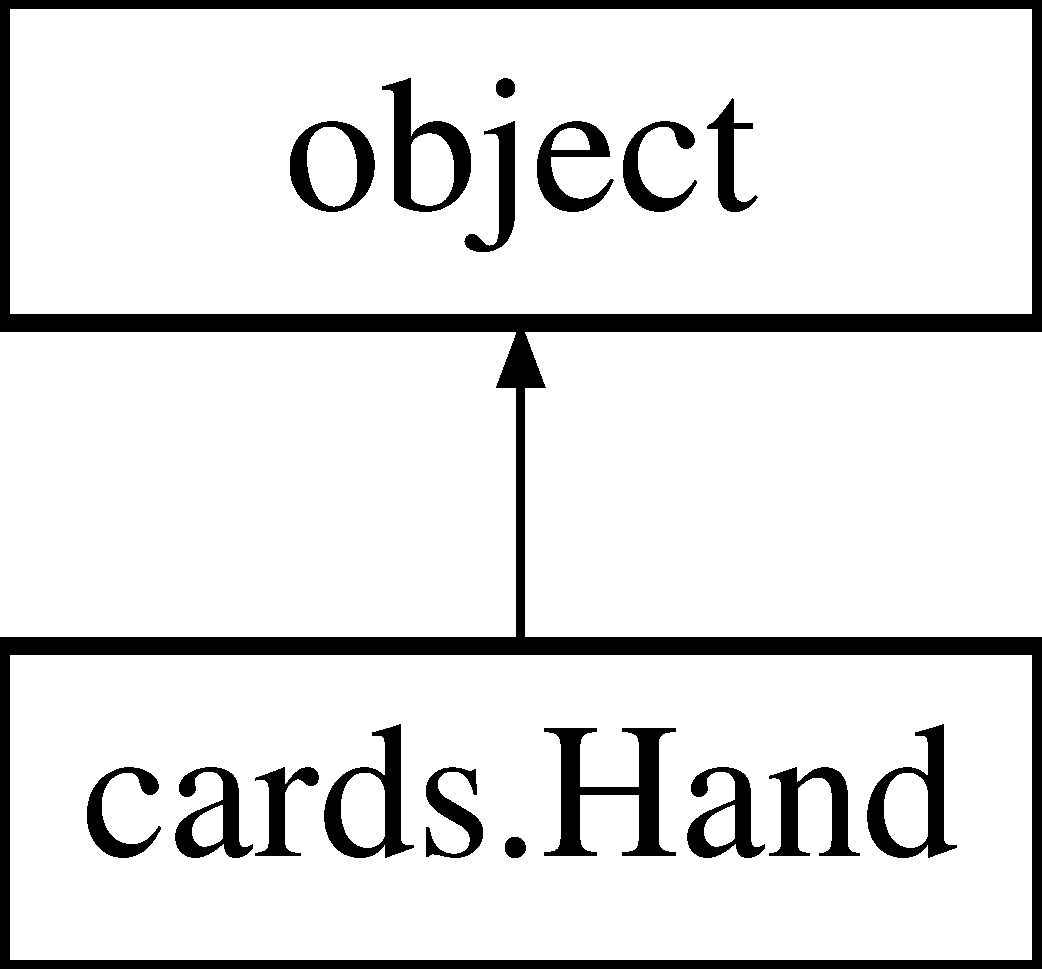
\includegraphics[height=2.000000cm]{classcards_1_1Hand}
\end{center}
\end{figure}
\subsection*{Public Member Functions}
\begin{DoxyCompactItemize}
\item 
def \hyperlink{classcards_1_1Hand_af800ad698281536204b51b71fb8ed15d}{\+\_\+\+\_\+init\+\_\+\+\_\+} (self, cards)
\item 
def \hyperlink{classcards_1_1Hand_a69f3ca64f85f68517e1aff96eecddf88}{n\+\_\+of\+\_\+a\+\_\+kind} (self, n)
\item 
def \hyperlink{classcards_1_1Hand_a6f47baa991d8cbc19de475dedc913c5d}{royal\+\_\+flush} (self)
\item 
def \hyperlink{classcards_1_1Hand_a968d069f9496b9be0b776cf556c9cc3e}{straight\+\_\+flush} (self)
\item 
def \hyperlink{classcards_1_1Hand_a154a7212af3b6230948078e83a5522a3}{four\+\_\+of\+\_\+a\+\_\+kind} (self)
\item 
def \hyperlink{classcards_1_1Hand_aa884f0c9ac8cb9e0d525fa6dd5f3b468}{full\+\_\+house} (self)
\item 
def \hyperlink{classcards_1_1Hand_a82d4acb563e208e8622948b436eceb60}{flush} (self)
\item 
def \hyperlink{classcards_1_1Hand_a29d0bc084338ab312ad249dc33e2f957}{straight} (self)
\item 
def \hyperlink{classcards_1_1Hand_a38deb8800110f1077223a605e5096cf2}{three\+\_\+of\+\_\+a\+\_\+kind} (self)
\item 
def \hyperlink{classcards_1_1Hand_a4bc879b8db18b48d745aecac892fa79c}{two\+\_\+pairs} (self)
\item 
def \hyperlink{classcards_1_1Hand_a0b6c8668a89a95ee985f475ae5b6775a}{one\+\_\+pair} (self)
\item 
def \hyperlink{classcards_1_1Hand_a52b92cc78391802ad2b9182bc326a403}{value} (self)
\item 
def \hyperlink{classcards_1_1Hand_a42ceab50738615707ec65667d1802496}{scoring\+\_\+cards} (self, score)
\item 
def \hyperlink{classcards_1_1Hand_aabc65985f97f74cefd0b550c3f47e652}{break\+\_\+tie} (self, other)
\item 
def \hyperlink{classcards_1_1Hand_a82fa918741361692526417b3295242dc}{\+\_\+\+\_\+lt\+\_\+\+\_\+} (self, other)
\item 
def \hyperlink{classcards_1_1Hand_a817ee76b140e59bf5c1e933283e5fb52}{\+\_\+\+\_\+le\+\_\+\+\_\+} (self, other)
\item 
def \hyperlink{classcards_1_1Hand_a1db1734329cd4a3be5a51447a1431646}{\+\_\+\+\_\+eq\+\_\+\+\_\+} (self, other)
\item 
def \hyperlink{classcards_1_1Hand_a35a85437e077522eef6448c863b6e570}{\+\_\+\+\_\+ne\+\_\+\+\_\+} (self, other)
\item 
def \hyperlink{classcards_1_1Hand_ae7d4f7a7e165bef7f32d6ed4c1781e6f}{\+\_\+\+\_\+gt\+\_\+\+\_\+} (self, other)
\item 
def \hyperlink{classcards_1_1Hand_a5d7400b5ff312926a03526db90acc22d}{\+\_\+\+\_\+ge\+\_\+\+\_\+} (self, other)
\end{DoxyCompactItemize}


\subsection{Constructor \& Destructor Documentation}
\hypertarget{classcards_1_1Hand_af800ad698281536204b51b71fb8ed15d}{}\index{cards\+::\+Hand@{cards\+::\+Hand}!\+\_\+\+\_\+init\+\_\+\+\_\+@{\+\_\+\+\_\+init\+\_\+\+\_\+}}
\index{\+\_\+\+\_\+init\+\_\+\+\_\+@{\+\_\+\+\_\+init\+\_\+\+\_\+}!cards\+::\+Hand@{cards\+::\+Hand}}
\subsubsection[{\+\_\+\+\_\+init\+\_\+\+\_\+}]{\setlength{\rightskip}{0pt plus 5cm}def cards.\+Hand.\+\_\+\+\_\+init\+\_\+\+\_\+ (
\begin{DoxyParamCaption}
\item[{}]{self, }
\item[{}]{cards}
\end{DoxyParamCaption}
)}\label{classcards_1_1Hand_af800ad698281536204b51b71fb8ed15d}


\subsection{Member Function Documentation}
\hypertarget{classcards_1_1Hand_a1db1734329cd4a3be5a51447a1431646}{}\index{cards\+::\+Hand@{cards\+::\+Hand}!\+\_\+\+\_\+eq\+\_\+\+\_\+@{\+\_\+\+\_\+eq\+\_\+\+\_\+}}
\index{\+\_\+\+\_\+eq\+\_\+\+\_\+@{\+\_\+\+\_\+eq\+\_\+\+\_\+}!cards\+::\+Hand@{cards\+::\+Hand}}
\subsubsection[{\+\_\+\+\_\+eq\+\_\+\+\_\+}]{\setlength{\rightskip}{0pt plus 5cm}def cards.\+Hand.\+\_\+\+\_\+eq\+\_\+\+\_\+ (
\begin{DoxyParamCaption}
\item[{}]{self, }
\item[{}]{other}
\end{DoxyParamCaption}
)}\label{classcards_1_1Hand_a1db1734329cd4a3be5a51447a1431646}
\hypertarget{classcards_1_1Hand_a5d7400b5ff312926a03526db90acc22d}{}\index{cards\+::\+Hand@{cards\+::\+Hand}!\+\_\+\+\_\+ge\+\_\+\+\_\+@{\+\_\+\+\_\+ge\+\_\+\+\_\+}}
\index{\+\_\+\+\_\+ge\+\_\+\+\_\+@{\+\_\+\+\_\+ge\+\_\+\+\_\+}!cards\+::\+Hand@{cards\+::\+Hand}}
\subsubsection[{\+\_\+\+\_\+ge\+\_\+\+\_\+}]{\setlength{\rightskip}{0pt plus 5cm}def cards.\+Hand.\+\_\+\+\_\+ge\+\_\+\+\_\+ (
\begin{DoxyParamCaption}
\item[{}]{self, }
\item[{}]{other}
\end{DoxyParamCaption}
)}\label{classcards_1_1Hand_a5d7400b5ff312926a03526db90acc22d}
\hypertarget{classcards_1_1Hand_ae7d4f7a7e165bef7f32d6ed4c1781e6f}{}\index{cards\+::\+Hand@{cards\+::\+Hand}!\+\_\+\+\_\+gt\+\_\+\+\_\+@{\+\_\+\+\_\+gt\+\_\+\+\_\+}}
\index{\+\_\+\+\_\+gt\+\_\+\+\_\+@{\+\_\+\+\_\+gt\+\_\+\+\_\+}!cards\+::\+Hand@{cards\+::\+Hand}}
\subsubsection[{\+\_\+\+\_\+gt\+\_\+\+\_\+}]{\setlength{\rightskip}{0pt plus 5cm}def cards.\+Hand.\+\_\+\+\_\+gt\+\_\+\+\_\+ (
\begin{DoxyParamCaption}
\item[{}]{self, }
\item[{}]{other}
\end{DoxyParamCaption}
)}\label{classcards_1_1Hand_ae7d4f7a7e165bef7f32d6ed4c1781e6f}
\hypertarget{classcards_1_1Hand_a817ee76b140e59bf5c1e933283e5fb52}{}\index{cards\+::\+Hand@{cards\+::\+Hand}!\+\_\+\+\_\+le\+\_\+\+\_\+@{\+\_\+\+\_\+le\+\_\+\+\_\+}}
\index{\+\_\+\+\_\+le\+\_\+\+\_\+@{\+\_\+\+\_\+le\+\_\+\+\_\+}!cards\+::\+Hand@{cards\+::\+Hand}}
\subsubsection[{\+\_\+\+\_\+le\+\_\+\+\_\+}]{\setlength{\rightskip}{0pt plus 5cm}def cards.\+Hand.\+\_\+\+\_\+le\+\_\+\+\_\+ (
\begin{DoxyParamCaption}
\item[{}]{self, }
\item[{}]{other}
\end{DoxyParamCaption}
)}\label{classcards_1_1Hand_a817ee76b140e59bf5c1e933283e5fb52}
\hypertarget{classcards_1_1Hand_a82fa918741361692526417b3295242dc}{}\index{cards\+::\+Hand@{cards\+::\+Hand}!\+\_\+\+\_\+lt\+\_\+\+\_\+@{\+\_\+\+\_\+lt\+\_\+\+\_\+}}
\index{\+\_\+\+\_\+lt\+\_\+\+\_\+@{\+\_\+\+\_\+lt\+\_\+\+\_\+}!cards\+::\+Hand@{cards\+::\+Hand}}
\subsubsection[{\+\_\+\+\_\+lt\+\_\+\+\_\+}]{\setlength{\rightskip}{0pt plus 5cm}def cards.\+Hand.\+\_\+\+\_\+lt\+\_\+\+\_\+ (
\begin{DoxyParamCaption}
\item[{}]{self, }
\item[{}]{other}
\end{DoxyParamCaption}
)}\label{classcards_1_1Hand_a82fa918741361692526417b3295242dc}
\hypertarget{classcards_1_1Hand_a35a85437e077522eef6448c863b6e570}{}\index{cards\+::\+Hand@{cards\+::\+Hand}!\+\_\+\+\_\+ne\+\_\+\+\_\+@{\+\_\+\+\_\+ne\+\_\+\+\_\+}}
\index{\+\_\+\+\_\+ne\+\_\+\+\_\+@{\+\_\+\+\_\+ne\+\_\+\+\_\+}!cards\+::\+Hand@{cards\+::\+Hand}}
\subsubsection[{\+\_\+\+\_\+ne\+\_\+\+\_\+}]{\setlength{\rightskip}{0pt plus 5cm}def cards.\+Hand.\+\_\+\+\_\+ne\+\_\+\+\_\+ (
\begin{DoxyParamCaption}
\item[{}]{self, }
\item[{}]{other}
\end{DoxyParamCaption}
)}\label{classcards_1_1Hand_a35a85437e077522eef6448c863b6e570}
\hypertarget{classcards_1_1Hand_aabc65985f97f74cefd0b550c3f47e652}{}\index{cards\+::\+Hand@{cards\+::\+Hand}!break\+\_\+tie@{break\+\_\+tie}}
\index{break\+\_\+tie@{break\+\_\+tie}!cards\+::\+Hand@{cards\+::\+Hand}}
\subsubsection[{break\+\_\+tie}]{\setlength{\rightskip}{0pt plus 5cm}def cards.\+Hand.\+break\+\_\+tie (
\begin{DoxyParamCaption}
\item[{}]{self, }
\item[{}]{other}
\end{DoxyParamCaption}
)}\label{classcards_1_1Hand_aabc65985f97f74cefd0b550c3f47e652}
\hypertarget{classcards_1_1Hand_a82d4acb563e208e8622948b436eceb60}{}\index{cards\+::\+Hand@{cards\+::\+Hand}!flush@{flush}}
\index{flush@{flush}!cards\+::\+Hand@{cards\+::\+Hand}}
\subsubsection[{flush}]{\setlength{\rightskip}{0pt plus 5cm}def cards.\+Hand.\+flush (
\begin{DoxyParamCaption}
\item[{}]{self}
\end{DoxyParamCaption}
)}\label{classcards_1_1Hand_a82d4acb563e208e8622948b436eceb60}
\hypertarget{classcards_1_1Hand_a154a7212af3b6230948078e83a5522a3}{}\index{cards\+::\+Hand@{cards\+::\+Hand}!four\+\_\+of\+\_\+a\+\_\+kind@{four\+\_\+of\+\_\+a\+\_\+kind}}
\index{four\+\_\+of\+\_\+a\+\_\+kind@{four\+\_\+of\+\_\+a\+\_\+kind}!cards\+::\+Hand@{cards\+::\+Hand}}
\subsubsection[{four\+\_\+of\+\_\+a\+\_\+kind}]{\setlength{\rightskip}{0pt plus 5cm}def cards.\+Hand.\+four\+\_\+of\+\_\+a\+\_\+kind (
\begin{DoxyParamCaption}
\item[{}]{self}
\end{DoxyParamCaption}
)}\label{classcards_1_1Hand_a154a7212af3b6230948078e83a5522a3}
\hypertarget{classcards_1_1Hand_aa884f0c9ac8cb9e0d525fa6dd5f3b468}{}\index{cards\+::\+Hand@{cards\+::\+Hand}!full\+\_\+house@{full\+\_\+house}}
\index{full\+\_\+house@{full\+\_\+house}!cards\+::\+Hand@{cards\+::\+Hand}}
\subsubsection[{full\+\_\+house}]{\setlength{\rightskip}{0pt plus 5cm}def cards.\+Hand.\+full\+\_\+house (
\begin{DoxyParamCaption}
\item[{}]{self}
\end{DoxyParamCaption}
)}\label{classcards_1_1Hand_aa884f0c9ac8cb9e0d525fa6dd5f3b468}
\hypertarget{classcards_1_1Hand_a69f3ca64f85f68517e1aff96eecddf88}{}\index{cards\+::\+Hand@{cards\+::\+Hand}!n\+\_\+of\+\_\+a\+\_\+kind@{n\+\_\+of\+\_\+a\+\_\+kind}}
\index{n\+\_\+of\+\_\+a\+\_\+kind@{n\+\_\+of\+\_\+a\+\_\+kind}!cards\+::\+Hand@{cards\+::\+Hand}}
\subsubsection[{n\+\_\+of\+\_\+a\+\_\+kind}]{\setlength{\rightskip}{0pt plus 5cm}def cards.\+Hand.\+n\+\_\+of\+\_\+a\+\_\+kind (
\begin{DoxyParamCaption}
\item[{}]{self, }
\item[{}]{n}
\end{DoxyParamCaption}
)}\label{classcards_1_1Hand_a69f3ca64f85f68517e1aff96eecddf88}
\hypertarget{classcards_1_1Hand_a0b6c8668a89a95ee985f475ae5b6775a}{}\index{cards\+::\+Hand@{cards\+::\+Hand}!one\+\_\+pair@{one\+\_\+pair}}
\index{one\+\_\+pair@{one\+\_\+pair}!cards\+::\+Hand@{cards\+::\+Hand}}
\subsubsection[{one\+\_\+pair}]{\setlength{\rightskip}{0pt plus 5cm}def cards.\+Hand.\+one\+\_\+pair (
\begin{DoxyParamCaption}
\item[{}]{self}
\end{DoxyParamCaption}
)}\label{classcards_1_1Hand_a0b6c8668a89a95ee985f475ae5b6775a}
\hypertarget{classcards_1_1Hand_a6f47baa991d8cbc19de475dedc913c5d}{}\index{cards\+::\+Hand@{cards\+::\+Hand}!royal\+\_\+flush@{royal\+\_\+flush}}
\index{royal\+\_\+flush@{royal\+\_\+flush}!cards\+::\+Hand@{cards\+::\+Hand}}
\subsubsection[{royal\+\_\+flush}]{\setlength{\rightskip}{0pt plus 5cm}def cards.\+Hand.\+royal\+\_\+flush (
\begin{DoxyParamCaption}
\item[{}]{self}
\end{DoxyParamCaption}
)}\label{classcards_1_1Hand_a6f47baa991d8cbc19de475dedc913c5d}
\hypertarget{classcards_1_1Hand_a42ceab50738615707ec65667d1802496}{}\index{cards\+::\+Hand@{cards\+::\+Hand}!scoring\+\_\+cards@{scoring\+\_\+cards}}
\index{scoring\+\_\+cards@{scoring\+\_\+cards}!cards\+::\+Hand@{cards\+::\+Hand}}
\subsubsection[{scoring\+\_\+cards}]{\setlength{\rightskip}{0pt plus 5cm}def cards.\+Hand.\+scoring\+\_\+cards (
\begin{DoxyParamCaption}
\item[{}]{self, }
\item[{}]{score}
\end{DoxyParamCaption}
)}\label{classcards_1_1Hand_a42ceab50738615707ec65667d1802496}
\hypertarget{classcards_1_1Hand_a29d0bc084338ab312ad249dc33e2f957}{}\index{cards\+::\+Hand@{cards\+::\+Hand}!straight@{straight}}
\index{straight@{straight}!cards\+::\+Hand@{cards\+::\+Hand}}
\subsubsection[{straight}]{\setlength{\rightskip}{0pt plus 5cm}def cards.\+Hand.\+straight (
\begin{DoxyParamCaption}
\item[{}]{self}
\end{DoxyParamCaption}
)}\label{classcards_1_1Hand_a29d0bc084338ab312ad249dc33e2f957}
\hypertarget{classcards_1_1Hand_a968d069f9496b9be0b776cf556c9cc3e}{}\index{cards\+::\+Hand@{cards\+::\+Hand}!straight\+\_\+flush@{straight\+\_\+flush}}
\index{straight\+\_\+flush@{straight\+\_\+flush}!cards\+::\+Hand@{cards\+::\+Hand}}
\subsubsection[{straight\+\_\+flush}]{\setlength{\rightskip}{0pt plus 5cm}def cards.\+Hand.\+straight\+\_\+flush (
\begin{DoxyParamCaption}
\item[{}]{self}
\end{DoxyParamCaption}
)}\label{classcards_1_1Hand_a968d069f9496b9be0b776cf556c9cc3e}
\hypertarget{classcards_1_1Hand_a38deb8800110f1077223a605e5096cf2}{}\index{cards\+::\+Hand@{cards\+::\+Hand}!three\+\_\+of\+\_\+a\+\_\+kind@{three\+\_\+of\+\_\+a\+\_\+kind}}
\index{three\+\_\+of\+\_\+a\+\_\+kind@{three\+\_\+of\+\_\+a\+\_\+kind}!cards\+::\+Hand@{cards\+::\+Hand}}
\subsubsection[{three\+\_\+of\+\_\+a\+\_\+kind}]{\setlength{\rightskip}{0pt plus 5cm}def cards.\+Hand.\+three\+\_\+of\+\_\+a\+\_\+kind (
\begin{DoxyParamCaption}
\item[{}]{self}
\end{DoxyParamCaption}
)}\label{classcards_1_1Hand_a38deb8800110f1077223a605e5096cf2}
\hypertarget{classcards_1_1Hand_a4bc879b8db18b48d745aecac892fa79c}{}\index{cards\+::\+Hand@{cards\+::\+Hand}!two\+\_\+pairs@{two\+\_\+pairs}}
\index{two\+\_\+pairs@{two\+\_\+pairs}!cards\+::\+Hand@{cards\+::\+Hand}}
\subsubsection[{two\+\_\+pairs}]{\setlength{\rightskip}{0pt plus 5cm}def cards.\+Hand.\+two\+\_\+pairs (
\begin{DoxyParamCaption}
\item[{}]{self}
\end{DoxyParamCaption}
)}\label{classcards_1_1Hand_a4bc879b8db18b48d745aecac892fa79c}
\hypertarget{classcards_1_1Hand_a52b92cc78391802ad2b9182bc326a403}{}\index{cards\+::\+Hand@{cards\+::\+Hand}!value@{value}}
\index{value@{value}!cards\+::\+Hand@{cards\+::\+Hand}}
\subsubsection[{value}]{\setlength{\rightskip}{0pt plus 5cm}def cards.\+Hand.\+value (
\begin{DoxyParamCaption}
\item[{}]{self}
\end{DoxyParamCaption}
)}\label{classcards_1_1Hand_a52b92cc78391802ad2b9182bc326a403}


The documentation for this class was generated from the following file\+:\begin{DoxyCompactItemize}
\item 
\hyperlink{cards_8py}{cards.\+py}\end{DoxyCompactItemize}


\subsection{File Documentation}
\label{sec:orgheadline21}
\hypertarget{cards_8py}{}\section{cards.\+py File Reference}
\label{cards_8py}\index{cards.\+py@{cards.\+py}}
\subsection*{Classes}
\begin{DoxyCompactItemize}
\item 
class \hyperlink{classcards_1_1Hand}{cards.\+Hand}
\end{DoxyCompactItemize}
\subsection*{Namespaces}
\begin{DoxyCompactItemize}
\item 
 \hyperlink{namespacecards}{cards}
\end{DoxyCompactItemize}
\subsection*{Functions}
\begin{DoxyCompactItemize}
\item 
def \hyperlink{namespacecards_ab58172fe17df72a0805b634ba5ec70fc}{cards.\+cards\+\_\+cmp} (a, b)
\item 
def \hyperlink{namespacecards_aca908702299162f0ce7ebed192ae90b2}{cards.\+denom} (card)
\end{DoxyCompactItemize}

\hypertarget{combinatorics_8py}{}\section{combinatorics.\+py File Reference}
\label{combinatorics_8py}\index{combinatorics.\+py@{combinatorics.\+py}}
\subsection*{Namespaces}
\begin{DoxyCompactItemize}
\item 
 \hyperlink{namespacecombinatorics}{combinatorics}
\end{DoxyCompactItemize}
\subsection*{Functions}
\begin{DoxyCompactItemize}
\item 
def \hyperlink{namespacecombinatorics_af4ad63ab1a68ba7c7efe8751623bc187}{combinatorics.\+fib} (n)
\item 
def \hyperlink{namespacecombinatorics_a14c14265f587c6fd4fc1bb9829ff5504}{combinatorics.\+digits} (n)
\item 
def \hyperlink{namespacecombinatorics_a37b7002188355ef3cac6f40cadb915ff}{combinatorics.\+nub} (nums)
\item 
def \hyperlink{namespacecombinatorics_a20423365036ac6b3e8560c994273e448}{combinatorics.\+has\+\_\+square} (n)
\end{DoxyCompactItemize}

\hypertarget{primes_8py}{}\section{primes.\+py File Reference}
\label{primes_8py}\index{primes.\+py@{primes.\+py}}
\subsection*{Namespaces}
\begin{DoxyCompactItemize}
\item 
 \hyperlink{namespaceprimes}{primes}
\end{DoxyCompactItemize}
\subsection*{Functions}
\begin{DoxyCompactItemize}
\item 
def \hyperlink{namespaceprimes_a27386dc3226d6aa9ec6ae476753d176f}{primes.\+primes\+\_\+seq} (n)
\item 
def \hyperlink{namespaceprimes_a7dffa5a7e9ee87a726e91e03a673282d}{primes.\+is\+\_\+next\+\_\+prime} (n, sieve)
\item 
def \hyperlink{namespaceprimes_a42460a84d6704d490f48e32fb5e5de66}{primes.\+is\+\_\+prime} (n, sieve)
\item 
def \hyperlink{namespaceprimes_a0fc2c4db3043a8d17dbd564ed9a3335e}{primes.\+next\+\_\+prime} (sieve)
\item 
def \hyperlink{namespaceprimes_afc18a8897a2405ada153fc92e27b4322}{primes.\+primes}
\item 
def \hyperlink{namespaceprimes_ae0a9ada316f92cba9ef0bad5495314fb}{primes.\+odd\+\_\+composite} ()
\item 
def \hyperlink{namespaceprimes_a8d1a9642a31428d166fdc5a8e400ce2a}{primes.\+factors} (n)
\end{DoxyCompactItemize}

\end{document}